\chapter{用户主观性建模}
\label{ch5}

\section{引言}
上一章介绍了如何对社交媒体中文档进行情感分类以确定文档表达的观点倾向性,本章将在上一章的基础上介绍用户层面的观点分析,主要包括如何对用户发表的多个文档中的观点信息进行集成,并以一种合理方式对集成的观点进行表示。

随着基于内容的社交媒体的兴起,越来越多的用户开始在社交媒体上针对各种话题发表短的文本信息表达意见和观点。本章研究的用户主观性是就是指用户感兴趣的话题(产品、政治人物和事件等等)以及用户对这些话题所持观点。一方面,社交媒体的文本数据因为覆盖话题广泛和用户观点信息丰富而成为研究用户主观性的重要数据来源。另外一方面,使用社交媒体数据研究用户的主观性反过来也会有利于针对社交媒体的后续研究及应用,比如用户观点查询、观点追踪或者用户行为的预测等研究,在社会学、心理学、政治以及商业领域具有重要作用。社交媒体中用户产生的内容数量巨大,而用户产生的文本信息短小分散,以碎片化形式存在于海量的社交媒体数据中,因此用户的主观性信息是散布在“碎片化的信息”中,使得从这些数据中挖掘和分析用户各种观点变得极具挑战性。例如,如果在Twitter中查询“iphone”(由于Twitter数据的实时流动性,不同时间查询会有不同的结果,此处结果查询日期为2014年2月14日),会返回大概231,233用户的830,879条微博(tweet,本文中统称为微博),意味着很多用户发表了不止一条微博来表达对“iphone”的观点。因此为了能够更好的了解到不同用户各种不同的观点,需要能够自动从用户发表的所有内容(UGC)中挖掘出“碎片化的观点”,将这些主观性信息进行集成(integrate),然后呈现出用户对于“iphone”这一感兴趣话题的整体观点\upcite{Lu2008}。实际上用户感兴趣的话题会有很多,发表的信息也是多种多样的,因此如何从一条条独立的“信息碎片”中找到用户感兴趣的话题和观点对用户主观性研究来说是很有意义的。

本章针对用户观点信息集成建模问题提出了主观性模型概念,在一个框架将话题和观点结合起来。主观模型分为两部分,一部分是用户感兴趣话题分布,用于用户对各种话题的兴趣度建模;另一部分是用户在每个话题上的观点分布,用于用户对话题发表的多个观点信息集成建模。图~\ref{fig5-1-1}展示了主观模型框架的总体结构,具体来讲,该框架通过三个步骤来解决用户话题观点集成问题:(1)首先使用用户层次的话题模型(user-level topic model)从用户发表的微博(以Twitter平台为例,当然该框架也可以适用于其他社交媒体平台)中抽取出用户感兴趣的话题;(2)使用话题模型和情感分析技术对用户每条微博进行话题和观点分析;(3)综合并集成用户所有微博的话题与观点信息形成用户的主观模型。

本章具体安排为:首先介绍相关工作,然后定义了用户层面的观点集成问题,接着给出主观模型定义以及构建方法,并以观点预测实际应用为例对主观模型进行了定性定量实验评测,最后是小节。

\section{相关工作}
\label{ch5_sec2}
虽然观点挖掘(Opinion mining)研究最先是在商品评论(Review)和新闻评论(Comment)\upcite{Pang2008OMS,Liu2012}领域兴起的,近年来越来越多的工作开始关注于Twitter等社交媒体短文本的观点信息,目前工作重点主要是针对单个短文本进行情感分析\upcite{Barbosa2010,Davidov2010,Jiang2011,Li2010,tan2011user},往往忽视了社交媒体的文本信息不是独立的,用户之间、数据之间以及用户与数据之间存在广泛联系。还有一些工作开始着眼于研究用户层面(User level)的主观性信息\upcite{Mostafa2013,Malouf2008},研究还主要是识别用户发表观点针对的目标\upcite{Liu2010}或是针对特定目标分析用户的观点倾向性\upcite{Zhai2011},而没有考虑到用户关心的多个话题、话题的各个方面(aspect)以及各方面观点的集成。自从Blei等\upcite{Blei2003}对文本的话题分析引入潜语义话题模型(Latent dirichlet allocation,LDA),开始有各种基于LDA的扩展模型用于从大规模语料中抽取用户的话题\upcite{Rosen-Zvi2004,Ramage2009},也有很多模型将情感分析与话题模型想结合设计话题情感模型(Topic-sentiment model),这种模型将情感极性与话题关联起来,代表性的主要有Mei等\upcite{Mei2007}的TSM模型和Lin等\upcite{Lin2009}的JST模型等,与本章提出的主观模型很接近,本章将与其进行定性和定量的分析对比。

随着用户在社交媒体上发布信息的增多,研究者因此能够获得越来越多的数据对用户建模(User modeling),这些用户模型对于用户行为分析等研究具有促进作用。例如Hannon等\upcite{Hannon2010}首先提出使用Twitter的社交网络关系以及用户微博内容对Twitter用户进行建模用于分析用户的转发微博行为;Macskassy和Michelson\upcite{Macskassy2011}使用Wikipedia作为外部知识库识别用户产生内容中的实体来对用户兴趣进行建模,并使用用户模型进行用户的分类研究;Ramage 等\upcite{Ramage2010}使用4S(Substance,Status,Style及Social)维度利用话题模型对用户的微博及社交关系分析建模,得到的模型在信息过滤和朋友推荐等应用中显示出了很好的效果;Xu等\upcite{Xu2012}提出了混合模型用于分析用户的发帖行为,混合模型将突发新闻、朋友发帖以及用户兴趣三个重要因素结合在一起预测用户的发帖行为;Pennacchiotti和Popescu~\upcite{Pennacchiotti2011}提出了一个综合各类信息对用户建模方法用于用户分类任务,确认了从用户产生内容中挖掘出的深层次特征的作用,方法反映了对用户及其网络结构的深入理解。

\begin{landscape}
\begin{figure*}[htb]
\centering
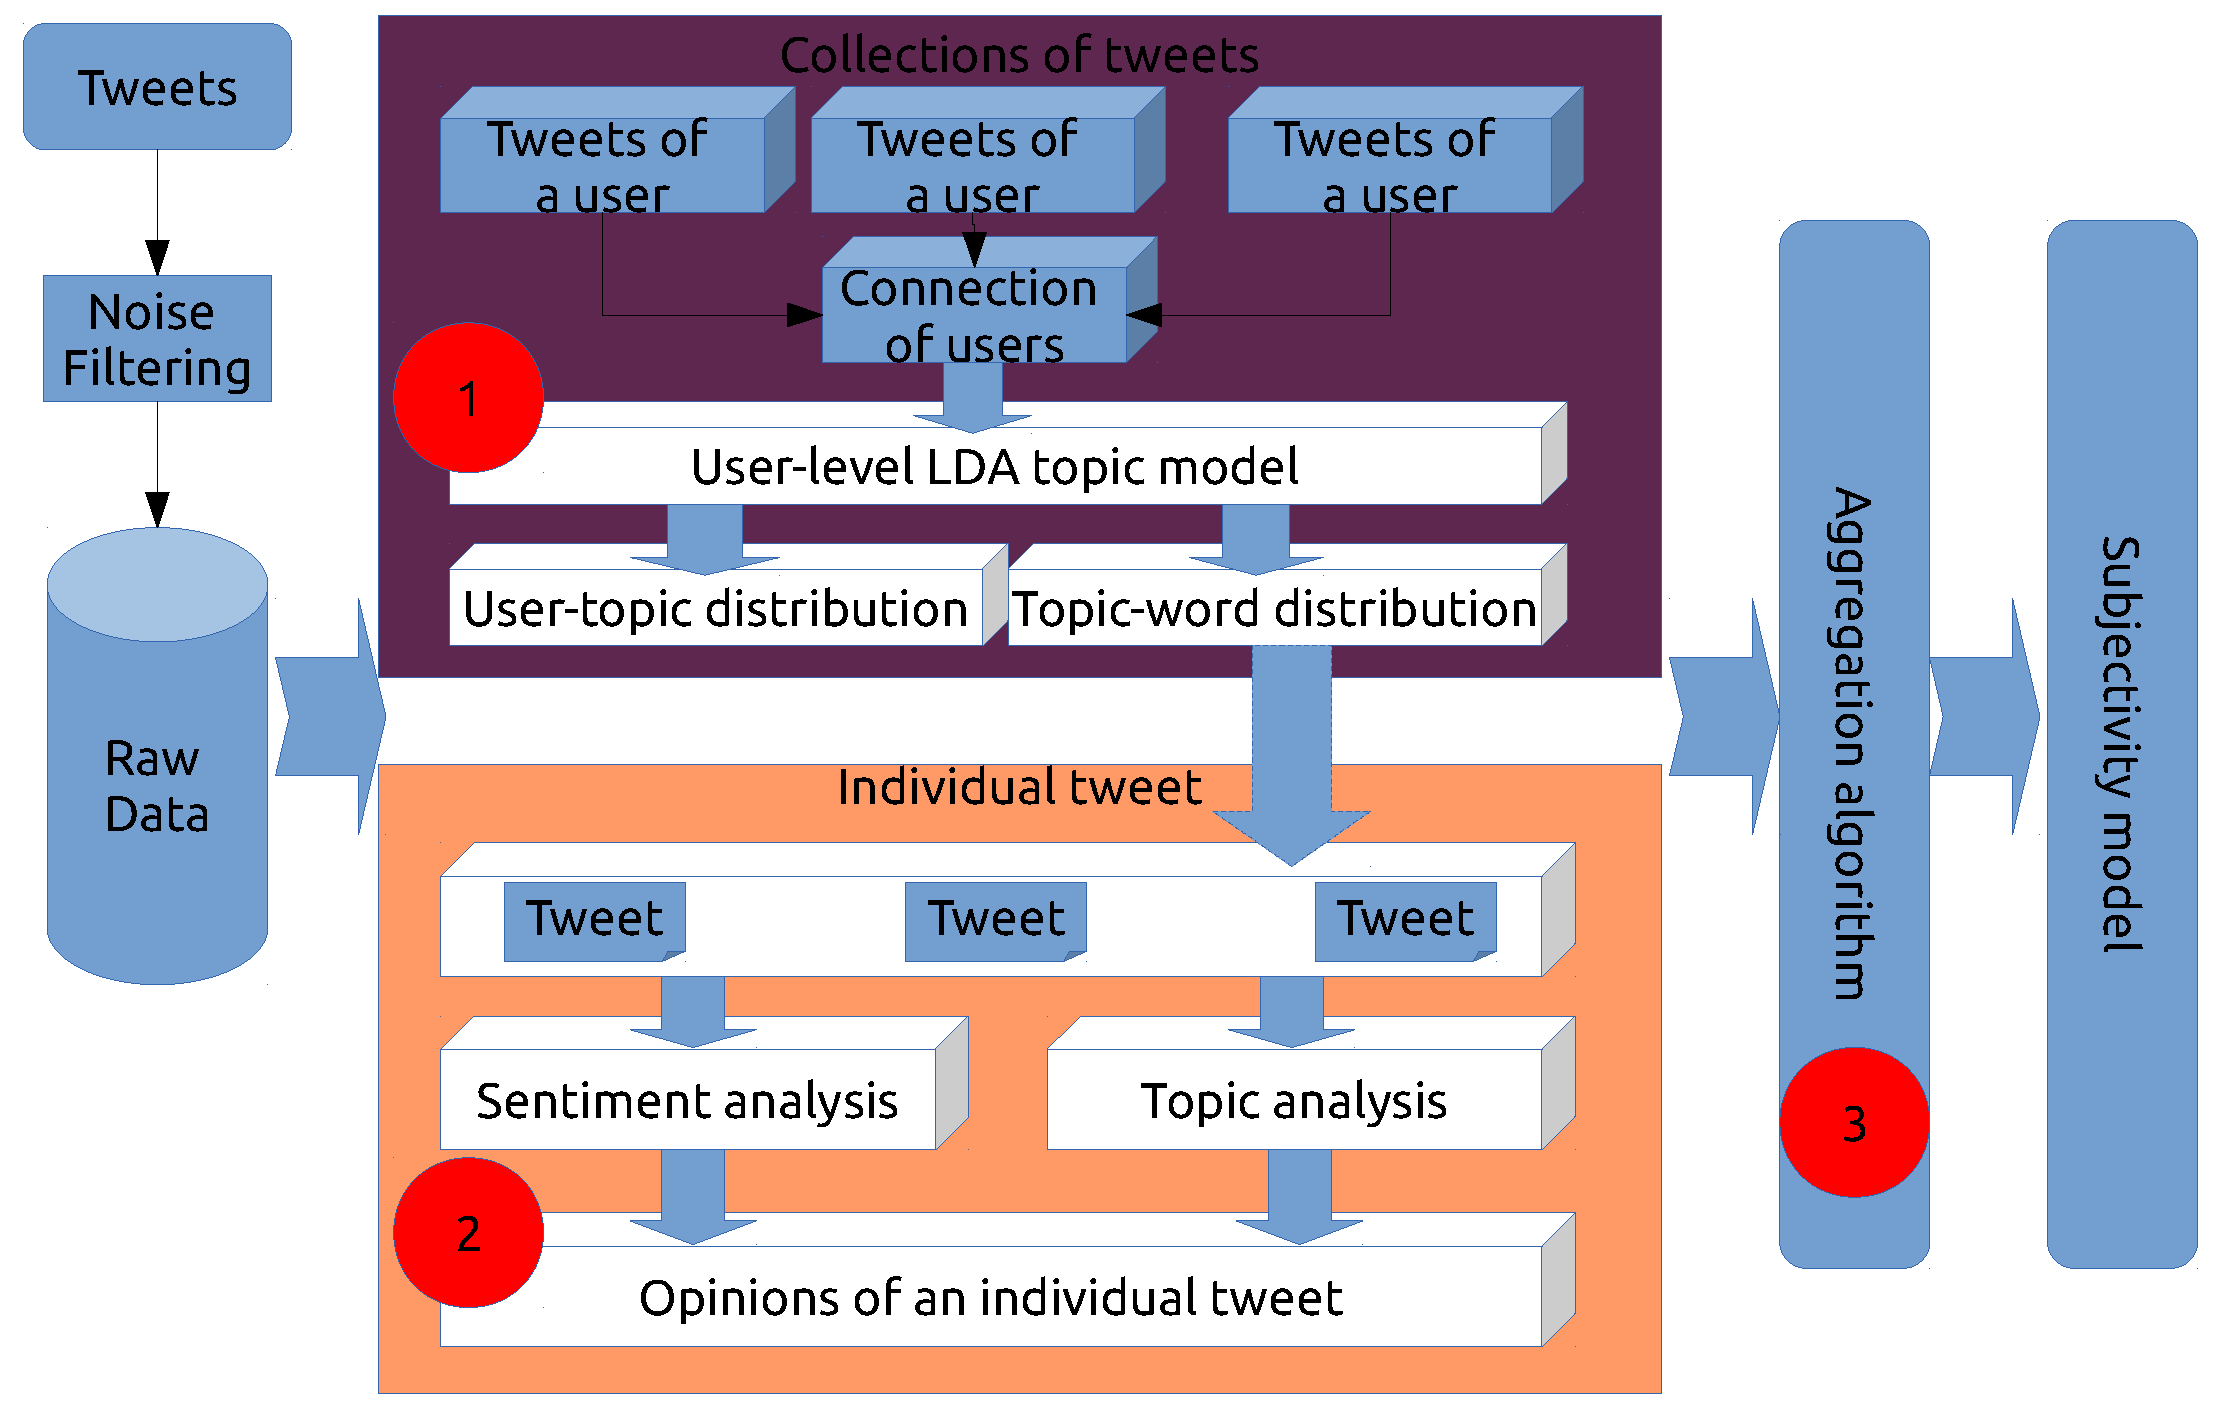
\includegraphics[height=300pt]{5-1.png}
\caption{主观模型总体框架}
\label{fig5-1-1}
\end{figure*}
\end{landscape}

上述这些工作都证明了从用户自己发布的内容中挖掘关键信息的重要性,并且从四方面信息对用户进行建模,即基本信息(“Who you are”),发帖行为(“How
you tweet”),发帖内容(“What you tweet”)以及网络关系(“Who you tweet”),但是少有工作关注于对用户的兴趣和观点进行综合建模,也就是全面反映用户的主观性,本章基于这一动机提出主观模型概念对用户的主观性进行建模。

\section{观点集成问题}
\label{sec3}
如在引言部分所介绍,用户在使用社交媒体平台的时候发布的信息是碎片化的信息,因为用户会在不同的时间就感兴趣的多个话题以及话题多个方面多次发表自己的观点。因此要确定一个用户在某个话题上观点不能只看他的一条信息,应该将他所有与特定话题相关的信息中的表达的观点进行综合才能确定用户的真正观点。为了满足对用户的主观性建模分析需求,在此提出观点集成问题(\textbf{Opinion Integration Problem} (OIP))定义作为用户层面的观点分析的基础。如果站在信息消费者角度,信息使用者主要关注用户层面(User level)的观点信息,而不是单个微博层面(tweet-level)的观点信息,因为观点分析的最终目标是发现人的主观想法而不只是单条微博中的观点信息,对单条微博中观点信息分析只是对分析用户主观性的一个中间步骤。此外,很多情况下用户的单条微博中的观点因为受到长度限制以及上下文语境的缺失常常是不明确的,但是通过用户的所有微博就可以知道其明确的观点信息\upcite{tan2011user}。

本节所提出的话题相关的观点集成问题(OIP)可以用图~\ref{fig5-2}进行说明。
\begin{figure}[htb]
\centering
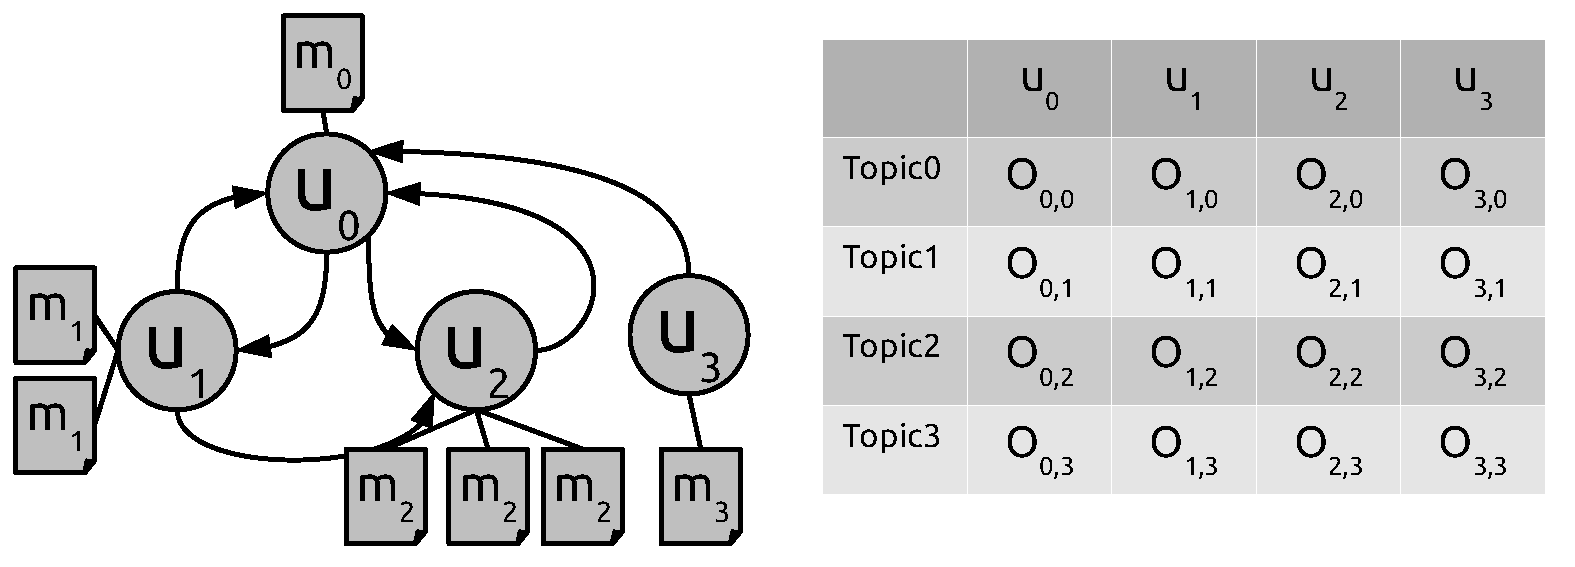
\includegraphics[height=130pt]{5-2.png}
\caption{观点集成问题示例}
\label{fig5-2}
\end{figure}
如图中所示,假设Twitter上的一个异构网络(heterogeneous network)是由用户集合$ V=\left\{ u_{i} \right\} $,用户之间的关系$ E=\left\{(u_{i},u_{j})| u_{i},u_{j} \in V\right\} $以及每个用户$ u_i $发表的微博集合$ M_{i}=\left\{ m_{i} \right\} $构成,其中用户所关注的话题$ T=\left\{ Topic_{j} \right\} $以及用户每条关于话题$ Topic_{j} $微博表达的观点$ o_{i,m,j} $可以从在网络中确定和抽取出来。于是观点集成问题可以定义为:
\begin{definition}[观点集成问题]
用户$ u_{i} $对某一话题 $ Topic_{j} $的观点$ O_{i,j} $不是他某条微博$ m_{i} $表达的观点,应该是从他所有与话题$ Topic_{j} $相关的微博$ M_{i}=\left\{ m_{i} \right\} $中通过某种方法$ f(o_{i,m,j}) $集成得出的,即:$$ O_(i,j)=\sum_mf(o_{i,m,j})$$
\end{definition}

观点集成问题有两个因素必须考虑:首先为了观点所针对目标话题的一致性,异构网络中无论是用户还是微博谈及的话题必须是在同一个话题空间,以使得无论话题的表示形式(比如概念(concept)表示或是话题模型的词袋向量空间的多项式分布表示)还是话题粒度都能够保持一致;其次,也是最重要的,就是集成的观点的表示形式问题,由于观点是与话题紧密相连的,一个用户针对某话题所发表的所有微博会覆盖与话题相关的所有方面,并且对于不同的方面会有不一样的喜好,比如对于手机“iphone”,用户可能喜欢它好看的外观和智能化操作系统,却不喜欢电池的待机时间过短,因此采用什么样的形式表示集成后的观点能准确表达出用户的总体观点是需要考虑的重要问题。下一节将会提出一个主观模型的概念,可以很好满足以上两个要求。

\section{主观模型}
\label{sec4}
其实心理学已经对主观性进行了广泛的研究,并基于个人的历史行为和言论中定义其主观性,以表示独特个性\upcite{Engbert2007}。在语言学上,语言中的主观性定义为作者在发布的文本中所表现出的自己立场、态度和情感\upcite{Stein2005}。社交媒体的出现为用户提供了能够针对感兴趣话题表达自己意见以展现自己独特主观性言论平台,因此在社交媒体平台上,用户的“\textbf{主观性}”可以定义为用户产生内容中涉及的话题和针对话题的表达的观点,因此主观性不但涉及到用户观点,也包含观点针对的目标。

本节首先给出主观模型的形式化定义以满足提出的用户层面观点分析需求。一般来讲,用户层面的观点分析是将用户针对某话题的情感极性分为“积极的(Positive)”或是“消极的(Negative)”。“积极的”情感表示该用户对话题支持或者喜欢,而“负面的”情感表示不支持或不喜欢。本节所提出的主观模型采用了更加通用(General)的“观点”定义,也就是用户针对某话题观点是一个在情感表示空间上的分布,该情感表示空间由可以表示情感强度的情感极性值构成。情感表达空间可以表示更细粒度的观点,因此可以更好的区分细致的观点差别,比如对话题持支持度为8的观点比支持度为5的观点更加具有“积极性”。其实对观点表示形式的定义还没有统一的标准,本节采用这种比较广义的定义是为了能使得主观模型能够更加通用。为了具体讨论问题,下面统一在Twitter平台对主观模型进行定义和分析,其实本章所提出的主观模型可以适用于其他的社交媒体平台。另外,之所以将模型命名为“\textbf{主观模型}”是因为是对社交媒体中用户产生内容中的主观性信息进行建模。

\subsection{模型定义}
\label{definition}
以$G=\left( V,E \right) $表示Twitter上一个异构社交网络,其中$ V $是网络中的用户,$ E\subset V\times V $是用户之间的关注关系(Following relationship)。对于每一个用户$ u \in V $,对应的微博集合 $ M_{u} $表示其发布所有内容。假设在这个社交网络中存在一个话题空间$ T $ 包含了$ V $中所有用户谈论的所有话题,以及一个情感表示空间$ S $用于表示用户观点。
对于用户$ u  \in V $的“\textbf{主观性(subjectivity)}”,定义为用户所发表的所有微博$ M_{u} $中所涉及的话题以及针对话题集成的观点。
  
\begin{definition}[主观模型]
用户$ u $的主观模型$ P \left( u \right) $是用户在话题空间$T$中所谈论话题$\left\lbrace  t \right\rbrace $以及他对每个话题所持有的观点$\left\lbrace O_{t}\right\rbrace $,观点用情感表示空间$ S $上的情感分布表示。
\begin{equation}
\label{usermodel}
P \left( u \right) = \lbrace \left( t, w_{u} \left( t \right), \lbrace d_{u,t} \left( s \right)|s \in S \rbrace \right) |  t \in T \rbrace
\end{equation}
其中:
\begin{itemize}
\item 对于用户$ u $,权重$ w_{u} \left( t \right)$表示其在话题空间中每个话题$t \in T$的兴趣强度,并且$ \sum_{t=1}^{|T|}w_{u} \left( t \right)=1 $。
\item 用户$ u $对话题$t$的观点$O_{t}$指的是对话题所有情感在情感强度空间$ S $的分布$O_{t}=\lbrace d_{u,t} \left( s \right)|s \in S \rbrace $,并且$ \sum_{s=1}^{|S|} d_{u,t} \left( s \right)=1$。
\end{itemize}
\end{definition}

主观模型通过将用户兴趣与观点同时考虑对用户的主观性进行建模,用户兴趣使用一个话题分布表示,对话题的观点用一个情感值的分布表示,主要目标是为了研究用户层面的观点信息,获得用户兴趣和观点比较全面的理解。

\subsection{主观模型的构建}
\label{establish}
根据主观模型的定义,使用了两个分布对用户的主观性进行建模:一个是话题分布,一个是针对每个话题的观点分布,二者都需要从用户发布的历史微博中经过计推理得出。然而对Twitter数据进行内容分析面临一些挑战:Twitter上微博数量十分庞大,但是每条微博由于受限于140字的限制而相对短小,并且各种不规范的语言被广泛使用,缺乏大规模的标注数据等。这些都使得机器学习方法和自然语言处理技术很难以达到好的分析效果\upcite{cambria2014jumping}。
因此能够有效的对Twitter的微博内容进行建模分析需要一些能应对这些挑战并且尽量不使用需要标注数据的方法和技术。为了主观模型的通用性,在设计构建方法时主要考虑使用一些无监督的技术从用户微博中挖掘话题和观点信息,然后通过观点集成来构建用户的主观模型。因此提出一个通用的框架来构建主观模型,该框架的主要优势就是利用Twitter的社交网络结构来帮助应对短文本微博造成的稀疏问题,并使用基于规则以及无监督方法解决无标注数据问题\upcite{Lin2010}。

\subsubsection{话题分析}
\label{topic}
微博所涉及的话题一般是隐性的,需要从微博内容中经过推导得出。目前针对微博话题发现研究主要集中于定位关键词(Key words)\upcite{Chen2010},抽取实体(Entity extraction)\upcite{Abel2011},借助外部知识库(External knowledge categories)\upcite{Macskassy2011},或者使用语义框架(Semantic framework)\upcite{Gangemi2014}等方法。这些方法面临一个主要的问题是数据稀疏问题,因为在谈论同一个话题时,不同用户会使用各种不同的词汇来描述和表达。还有一个重要的方向是各种无监督话题模型,其中LDA话题模型\upcite{Blei2003}及其各种扩展模型\upcite{Weng2010}对微博中的话题分析更加有效\upcite{Hong2010}。LDA模型的话题表示形式在概念上更加宽泛,每一个话题都表示为在所有词空间上的一个分布,因此可以有效应对话题表示的稀疏问题。主观模型的构建框架采用了用户层面LDA话题模型(User-level LDA)从用户所有的微博中发现隐性话题,对应于LDA话题模型,用户层面LDA话题模型生成过程可以使用图~\ref{fig5-1}来表示。

\begin{figure}[htb]
\centering
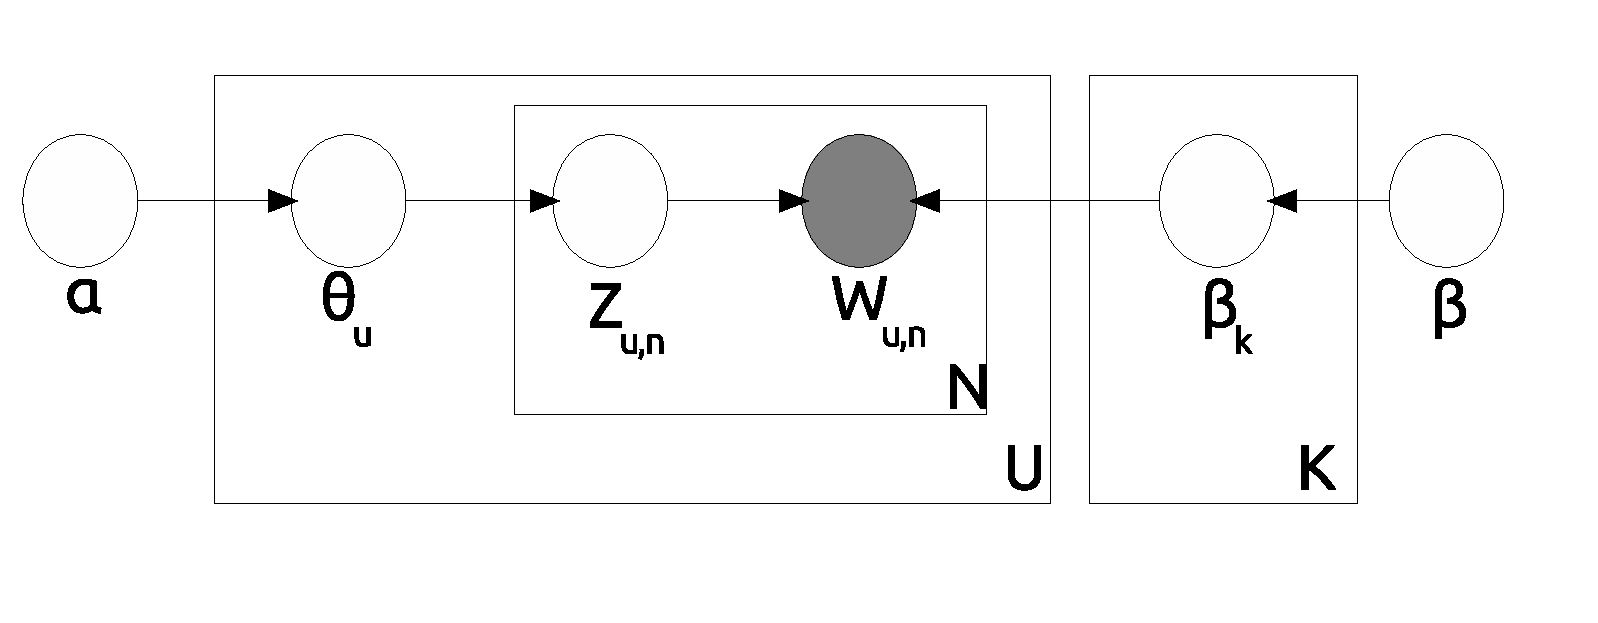
\includegraphics[height=100pt]{5-0.eps}
\caption{用户层面LDA话题模型}
\label{fig5-1}
\end{figure}

具体生成过程如下:
\begin{itemize}
\item 对每个用户$ u $,从先验中获取兴趣话题分布$ \theta_{u} \sim Dir \left(  \alpha \right) $;
\item 对用户微博中的每个词语$ w_{u,n} $,$ n \in \left\lbrace 1, \cdots, N \right\rbrace $:
\begin{itemize}
\item 从用户兴趣话题分布中获取一个话题$ z_{u,n} \sim Multinomial \left( \theta_{u}  \right) $;
\item 根据话题$ z_{u,n} $,从话题的多项分布中获取词语$ w_{u,n} $:$ p \left( w_{u,n} \vert z_{u,n}, \beta_{k}  \right) $。
\end{itemize}
\end{itemize}

为了从用户产生的内容中抽取出涉及的话题,用户产生的微博内容应该和LDA话题模型的文档对应起来。构建主观模型时,主要目标是为了了解用户感兴趣的话题而不是单条微博谈论的过细话题,所以我们将每一个用户的所有微博连接起来组成一篇微博文档作为LDA模型的输入文档。因此用户层面LDA模型中的一篇文档就对应于一个用户,一个用户感兴趣的话题可以使用在话题空间的一个多项式分布来表示,分布的权重可以和主观模型的话题权重相对应。形式化表示为:在用户层面的LDA模型中,给定用户集合$ V $以及话题数目$ K $,一个用户$ u \in V $的所有微博文档可使用话题上一个多项分布$ \theta_{u} $来表示,该分布具有参数为$ \alpha $的Dirichlet先验分布;一个话题$ k \in K $可以用所有词汇上的一个多项分布$ \beta_{k} $来表示,该分布具有参数为$ \eta $的Dirichlet先验分布。模型中的两个分布能够使用Gibbs采样或变分推理(Variational inference)方法进行估计。构建框架中实际本章中我们使用的是基于变分推理的话题模型工具Gensim\upcite{vRehruvrek2010},该工具使用的是在线批处理模式的变分推理方法。

\subsubsection{观点分析}
\label{sentiment}
微博用户经常会通过发表一些跟自己感兴趣话题相关的微博来表达自己的观点,因此为了分析微博用户的主观性,需要了解用户每条微博表达的观点。前面三章内容详细介绍了社交媒体观点分析的各种方法,主要方法可以分为基于规则(词典)方法以及基于机器学习方法两类。如果要准确分析微博观点,基于机器学习方法训练过程需要大量标注数据,Twitter的庞大数据量以及语言的动态性决定了很难对这样的数据进行标注,主观模型的构建优先采用基于规则的方法,基于规则的方法具有很好的灵活性,可以将Twitter的一些语言特点转化成为分析规则,因而更适用于Twitter的观点分析\upcite{Hu2013,Thelwall2010}。

在基于规则的方法中,SentiStrength是专门针对社交媒体中的不规范短文本数据进行情感分析的工具包\upcite{Thelwall2010}。SentiStrength将对应于社交媒体语言特点的规则融合进了基于词典的方法,非常适用于主观模型对Twitter观点分析需求。SentiStrength对每条微博情感分析后输出两个情感值:一个积极极性情感强度值($ [1,5] $范围内)和一个消极极性情感强度值($ [-5,-1] $范围内)。SentiStrength输出的情感值不是简单的积极和消极极性二值结果,而是细粒度的情感强度值,符合主观模型细粒度情感表示空间上分布需求。因此主观模型构建框架使用SentiStrength对所有微博进行情感分析。为了使用方便,将SentiStrength的两个输出结果映射为一个在$ [0, 8] $的离散整数值表示情感强度,映射函数为:
\begin{equation}
\label{opinionmap}
o=\begin{cases} 
{p+3} &  \qquad if \; \vert p \vert > \vert n \vert \\
{n+5} &  \qquad if \; \vert n \vert > \vert p \vert \\
{4}  &   \qquad if \; \vert p \vert = \vert n \vert
\end{cases}
\end{equation}
其中$ p $代表SentiStrength输出的积极极性情感强度值,$ n $代表消极极性情感强度值。与情感极性想对应,在$ [0, 8] $情感表示空间中,强度值4和5表示中性(neutral)情感,强度值大于5表示积极极性,强度值小于4表示消极极性。使用SentiStrength对用户的每条微博进行情感分析的到一个在$ [0, 8] $情感表示空间的情感值,将所有微博的情感值综合,就可以对用户的观点进行集成。

\subsubsection{构建主观模型}
\label{concrete}
对用户微博进行话题分析以及情感分析后,我们就可以为用户开始构建主观模型了。
对于一社交网络的用户集合$ V $,用$ M_{u}=\left\lbrace m_{i} \right\rbrace$表示每一用户 $ u \in V $所发布的所有微博。按照用户层面LDA话题模型要求,将$ M_{u} $中所有微博连接在一起形成一片长的微博文档$ d_{u} $,然后可以用这些微博文档$\{ d_{u}|u \in V\} $使用LDA话题模型进行训练获得话题个数为$ K $的话题空间。
训练得到的话题模型用参数$ \theta $表示每个用户在话题空间$ T $中感兴趣的话题的分布,参数$ \beta $表示每个话题在所有微博词汇上的分布。
使用SentiStrength对每个用户的每条微博$ m $进行情感分析得到每条微博大的情感强度$ s_{m} $。用户主观模型的构建过程可以分为三个步骤:
\begin{enumerate}
\item 在生成的话题模型中,参数$ \theta_u $可以直接对应到用户$ u $在话题空间中的兴趣话题分布,可以确定用户感兴趣话题为:
\begin{equation}
\label{eq5-1}
Z_u=\{t|p(t|\theta_u(t))>0,t \in T\}
\end{equation}
\item 将话题模型应用到用户$ u $每条微博$ m $确定涉及话题为:
\begin{equation}
\label{eq5-2}
Z_m=\{t|p(t|\theta,\beta,m)>0,t \in T\}
\end{equation}
\item 对用户$ u $发布的所有涉及话题$ t $的微博观点进行集成分析的到用户在话题上的观点:
\begin{equation}
\label{eq5-3}
O_{t} = \left\{ \frac{N_{s}}{\sum_{s \in S} N_{s}} |s \in [0,8] \right\}
\end{equation}
其中$ N_s =\sum_{m \in M_{u}} I\left( s_{m} \right) $($s_{m}=s \& t \in Z_{m} $)表示用户发布的涉及话题$ t $情感值为$ s $微博数目。

最后综合形成用户主观模型:
\begin{equation}
\label{subuser}
P(u)= \left\lbrace \left( t, p\left( t \vert \theta_{u} \right), \left\{ \frac{N_{s}}{\sum_{s \in S} N_{s}} \right\}  \right)  \vert t \in Z_{u}, s \in S  \right\rbrace
\end{equation}
\end{enumerate}

对用户$ u $构建主观模型$ P(u) $的详细过程如算法~\ref{alg5-1}所示:

\begin{algorithm}[htb] 
\caption{主观模型的构建过程} 
\label{alg5-1}
\begin{algorithmic}[1] %这个1 表示每一行都显示数字
\REQUIRE ~~\\ %算法的输入参数:Input
用户集合$ V $;\\
每个用户所发布的微博集合 $ M_{u} $;\\
\ENSURE ~~\\ %算法的输出:Output
为每个用户$ u $构建的主观模型 $ P(u) $;
\STATE 使用用户层面的话题模型对用户微博内容分析获得模型 $P(\theta,\beta|M_{u},V)$; 
\label{ alg1:topic }%对此行的标记,方便在文中引用算法的某个步骤
\FORALL {用户每条微博 $ m \in M_{u} $}
\label{alg1:sentiment}
\STATE 对 $ m $情感分析获得情感值 $ s_{m} $;
\ENDFOR
\FOR {每个用户$ u \in V$}
\STATE 用户感兴趣话题分布为参数$ \theta $对应的分布 $ \theta_{u} $;\\
\STATE 使用公式~\ref{eq5-1}确定用户话题集合$ Z_{u}$;
\ENDFOR
\FOR {每条微博 $ m \in M_{u} $}
\STATE 使用公式~\ref{eq5-2}对微博$ m $话题分析,得到微博涉及话题$ Z_m $;
\ENDFOR
\FOR {用户每个兴趣话题$ t \in Z_{u} $ }
\FOR {情感表示空间的每个情感值$ s \in S $}
\STATE 统计用户$ u $发布的微博中情感值为$ s $且涉及话题$ t $的数目$ N_{s}$;
\ENDFOR
\STATE 使用公式~\ref{eq5-3}计算用户$ u $对话题$ t $的集成的观点分布$ O_t $;
\ENDFOR
\STATE 构建用户$ u $的主观模型$  P(u)$;
\RETURN $P(u)$ %算法的返回值
\end{algorithmic}
\end{algorithm}

以上的构建方法中,由于微博话题的集中性,简单假设微博$ m $的情感$ s_m $是针对微博所涉及的所有话题$ Z_{m} $,并没有区分针对不同话题的不同情感。

\subsection{与生成模型比较}
\label{comparison}
在情感分析领域,一些研究提出了基于话题模型的话题情感模型,能够扩展基本的话题模型将文档中表达的情感与话题相结合统一建模\upcite{Mei2007,Lin2009}。其中TSM模型(Topic Sentiment Mixture model)\upcite{Mei2007}认为文档中表示情感等主观信息的词语与描述话题的词语是相互独立的,因此可以将表示情感的语言模型跟表示话题的语言模型分开建模,在文档的生成过程中任一词语的生成或者从话题语言模型中采样获得,或者从情感语言模型中采样获得,二者只能选择一个。JST模型(Joint Sentiment/Topic model)\upcite{Lin2009}提出了一种新的方式来分析文档中的情感信息,在话题模型抽取话题过程中将话题和情感关联起来,因此可以同时对话题和情感信息联合建模。
这些模型在发现话题相关的情感极性时跟本章提出的主观模型是很相似的,都能同时对用户的感兴趣话题以及话题相关的主观性信息建模。

但是这类模型通常假设存在一个词语-情感分布,需要通过学习获得这个通用词语-情感分布来对文档中的情感知识建模,这对短小和不规范社交媒体语言,尤其是Twitter来说是很困难的。相对于话题的表达,情感、观点等主观信息更难识别,因为情感信息常常隐式的存在于一些微妙的语言表达方式中(比如反讽),并且一些具体的领域和语境中也会具有独特的情感表达方式。微博中的情感除了一些正规语言的表达方式外,还有很多微博特有的语言来表达,比如表情符、字母大小写变化、不规范词语中字母重复强调以及惊叹号等标点符号的使用等等。微博上的这些语言特点表达出的情感很难用词语-情感概率分布表示。但是基于规则的情感分析方法可以很容易通过设计规则反映这些特有语言特点,用规则获取微博语言中微妙的情感表达方式。因此,主观模型构建中采用了基于规则的情感分析工具发现微博中的情感信息,更适合于Twitter等短文本社交媒体上用户主观性的建模。

\subsection{主观模型的应用}
\label{application}
从用户微博中学习得到的主观模型能够应用到用户观点分析以及行为(转发、关注等行为)分析中。本节以用户观点的预测为例来验证主观模型的作用,也就是学习到的主观模型能否有效的对用户将来针对某话题的观点进行预测。根据用户观点的一致性,假设用户不会就某一话题随机表达积极或消极极性观点,例如一个支持某候选人的用户更趋向于针对该候选人发表正面观点的微博。社会学上称这种现象为人的主观偏执(bias),也就是人的主观性\upcite{Walton1991}。因此得到了用户的主观模型,可以根据用户前期表现出的主观性预测用户就某一话题发表的微博所持观点。

首先将这种观点预测问题形式化为三元组$ < author, m, t >$,其中$author$是微博$ m $作者,微博涉及话题为$ t $。观点预测的目标就是通过计算得出用户$author$的微博$ m $针对话题$ t $表达出的观点极性$ p=\left\{positive,negative\right\} $。情感分析领域针对这一问题的主要方法是从微博中抽取出文本的情感表达模式,然后利用这些模式来预测观点的极性。
单条微博经常会由于缺乏上下文信息而使得观点具有模糊性,用户的主观模型是从用户所有的历史微博中构建的,因此有丰富的上下文信息,并且根据用户主观性的一致性假设,主观模型中对某一话题的观点比一条微博中的观点更加稳定一致。因此可以使用主观模型来提高用户未来发表微博中观点预测效果。
具体来说,对微博$ m $,其作者的主观模型可以根据算法~\ref{alg5-1}构建,假设作者新发布的微博为$ m $,$ m $的情感值通过某种方法比如SentiStrength分析得出为$s_m$,并且$ m $所涉及话题可以使用的公式~\ref{eq5-4}推导得出:
\begin{equation}
\label{eq5-4}
\hat{t}=argmax(\hat{P}(t| \theta,\beta ,Z_{u})|t)
\end{equation}

用户$author$在话题$ \hat{t} $上的观点分布可以从主观模型$ P(author) $中确定为$ O_{author,\widehat{t}} $,是一个在情感表示空间$ S $上的分布,因此可以计算出用户在话题$ \hat{t} $上归一化情感值:
\begin{equation}
\hat{s_{m}}=\sum_{i \in T}d_{i}\ast v_{i}
\end{equation}
其中$ v_{i} $表示情感值,$ d_{i} $表示情感值对应的分布。

于是可以使用微博情感分析得到的情感值$s_m$和主观模型计算出的情感值$ \hat{s_{m}} $联合进行观点极性$ p $预测:

\begin{equation}
\label{polarity}
p=  
\begin{cases}
{positive} &  \qquad if \; \dfrac{\hat{s_{m}}+s_m}{2} > \dfrac{|S|}{2} +1\\
{negative} &  \qquad if \; \dfrac{\hat{s_{m}}+s_m}{2} < \dfrac{|S|}{2} \\
{neutral}  &   \qquad otherwise \;  
\end{cases}
\end{equation}

\section{实验}
\label{sec5}

\subsection{数据集及设置}
实验使用的数据集是通过Twitter公开API抓取的数据集\upcite{Li2012a},数据集的具体规模如表~\ref{tab5-1}所示。

\begin{table}
\centering
\caption{Twitter数据集统计}
\label{tab5-1}
\begin{tabular}{|l|l|l|l|}
\hline
项目 & 规模 & 项目 & 规模\\
\hline
总用户数& 139,180 & 每个用户平均朋友数& 14.8 \\
\hline
总连接数 &  4,175,405 & 每个用户平均粉丝数 & 14.9  \\
\hline
总微博数 & 76,409,820 & 每个用户平均微博数 & 549 \\
\hline
\end{tabular}
\end{table}

由于LDA模型的计算复杂度,直接从139,180个用户的所有微博中构建主观模型需要大量时空开销。根据社交网络的同质性(Homophily)\upcite{Lazarsfeld1954},也就是“物以类聚(Birds of a feather flock together)”的原则\upcite{McPherson2001},社交网络中连接紧密的用户更趋向于讨论相同话题,持有相似观点\upcite{Thelwall2010a}。在Twitter上,用户之间的连接关系对应着用户间的认可或关注关系,还意味着拥有有相似话题或观点。因此可以利用社交网络的连接紧密用户形成的社区结构(community),将139,180个用户划分为不同的社区,在社区内部为用户构建主观模型,这种利用社交网络结构特点化整为零的方法,可以降低构建主观模型的计算复杂度。实验使用Igraph\footnote{\url{http://igraph.org/}}工具包划分社区,最后将用户划分为106个社区。对于用户数少于15的小社区,使用LDA模型进行话题分析效果比较差,因此实验中将这些社区和用户过滤,同时也过滤掉了发微博少于5的、每次发微博字数少于5个的还有微博内容只有url连接的用户总共15,756个。最后形成的数据集中有122,329个用户,分部于33个社区中。每个用户在其社区内局部网络中按照算法~\ref{alg5-1}构建主观模型。

除了主观模型,实验也将主观模型与两个话题情感生成模型JST和TSM进行了对比试验。所有模型的Dirichlet先验参数设为$ \alpha=50/T $($ T $为话题数目),$ \beta=0.01 $。JST的不对称情感先验参数$ \gamma $依照经验设为$ (0.01, 1.8) $。JST和TSM模型推导都经过了2,000次迭代Gibbs采样。

\subsection{样例分析}
为了定性展主观模型表达用户主观性能力,在此给出了使用本章提出框架构建的一个用户的主观模型如图~\ref{fig5:a}和~\ref{fig5:b}所示。该用户发表了533条微博,所有微博可以用词云图\footnote{实验使用TagCrowd (\url{http://tagcrowd.com/})生成词云图。}~\ref{fig5:a}来展示。

\begin{figure}[htb]
\centering
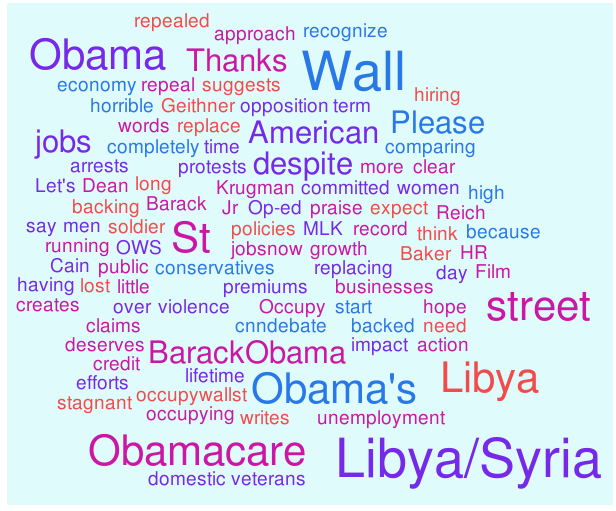
\includegraphics[height=220pt]{5-4.png}
\caption{微博词云}
\label{fig5:a}
\end{figure}

\begin{figure}[htb]
\centering
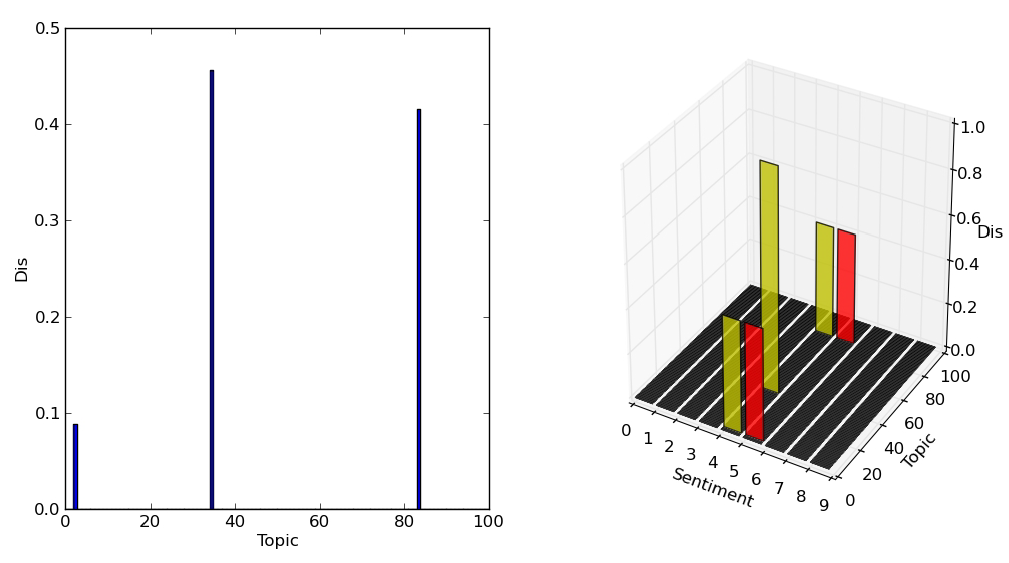
\includegraphics[height=200pt]{5-3.png}
\caption{主观模型样例}
\label{fig5:b}
\end{figure}

图~\ref{fig5:b}\footnote{主观模型中,左侧图代表话题分部: $ (  w_{u}\left( 2 \right)=0.08,w_{u}\left( 32 \right)=0.48, w_{u}\left( 83 \right)=0.44)  $;右侧图代表观点的分部: $ O_{2}=( d_{u,2} \left( 4 \right)=0.5, d_{u,2} \left( 5 \right)=0.5)$, $O_{32}=(d_{u,32} \left( 4 \right)=1.0) $, $ O_{83}=( d_{u,83} \left( 4 \right)=0.5, d_{u,83} \left( 5 \right)=0.5 ) $。}是用户在$ [0,100] $话题空间和$ [0,8] $情感表示空间中可视化的主观模型。很明显,从词云图上可以看到该用户讨论了三个话题(话题2:``\#Obamacare'',话题32:``\#libya''以及话题83:``\#occupywallst''),图~\ref{fig5:b}左侧展示了用户在每个话题上的兴趣权重。图~\ref{fig5:b}右侧是用户对这三个话题所持观点分布,总体来看,对于话题``\#libya''情感分布100\%在强度4上,属于中性,对话题``\#Obamacare''和``\#occupywallst''情感分部都是50\%在强度4以及50\%在强度5上,属于中性偏积极极性。从这个样例可以看出,主观模型对用户的主观性进行了细致的建模,不但有用户的兴趣分布,也有细粒度的观点分布信息。

\subsection{观点预测性能}
为了定量评价主观模型的性能,主观模型在观点预测任务上与两个话题情感模型(TSM和JST)以及几个常用的情感分析方法进行了对比实验。由于缺少可用的标注数据,实验中主要跟几个无监督的情感分析方法进行了对比,这些方法主要有:
\begin{itemize}
\item \textbf{OF:OpinionFinder}是一个公开可用的情感分析软件包,主要是用于句子层面的主观性分析\upcite{Wilson2005}。
\item \textbf{S140:Sentiment140}使用远距离监督(distant supervision)方式(使用表情符获取训练数据)进行微博的情感分类的在线工具。
\item \textbf{STR:SentiStrength}将微博中的一些语言特点转化成规则,并结合基于情感词典方法,专门针对微博等社交媒体短文本进行情感分析工具\upcite{Thelwall2010}。
\end{itemize}

实验从数据集中随机选择了1,000个至少有80条微博的用户,然后选择每个用户按照时间顺序发布的最后一条微博组成了1,000条测试数据集。所有的1,000条微博进行人工标注作为评测标准。话题模型的话题数分别设置为50, 100, 150以及200,评价指标使用的是准确率,结果如表~\ref{tab5-2}所示。

\begin{table}[htb]
\centering
\caption{观点预测对比实验结果}
\label{tab5-2}
\begin{tabular}{|l|l|l|l|l|}
\hline
情感分类方法 & 50 & 100 & 150 & 200\\
\hline
OF &  65.85\%& & & \\
\hline
S140 &  70.45\%& & & \\\hline
STR &  69.98\%& & & \\\hline
TSM & 63.46\%& 72.94\% $ \ast $  &67.83\% & 66.65\% \\\hline
JST & 61.25\% & 68.57\% $ \ast $ & 75.88\%  $ \ast $ & 67.03\%\\\hline
SUB & 71.53\% $ \ast $ & 81.05\% $ \ast $ & 78.32\% & 74.54\%\\
\hline
\end{tabular}
\begin{tablenotes}
  \centering
  \footnotesize
  \item 相对于OF显著的性能提升使用$ \ast $标记。\\
\end{tablenotes}
\end{table}

从表中可以看出:
\begin{itemize}
\item 首先,OpinioFinder的准确率是最低的65.85\%,主要原因是OpinioFinder主要是针对评论而设计的情感分析工具,不适用于Twitter这种语言环境;
\item 其次,两个无监督情感分析方法Sentiment140和SentiStrength因为是专门针对Twitter设计,准确率都明显好于OpinionFinder(Sentiment140:70.45\%,SentiStrength:69.98\%);
\item 第三点,总体上两个话题情感生成模型TSM和JST的准确率都好于OpinioFinder,并且准确率都比Sentiment140和SentiStrength方法稍好(但是不显著),证明了将情感信息与话题分析相关联的重要性;
\item 最后,主观模型(SUB)准确率在四种话题设置下准确率都显著地好于三个无监督情感分析方法,并且将主观模型计算出的情感值与SentiStrength对微博情感值想结合后,显著提高了SentiStrength准确率,与两个话题情感生成模型相比较,主观模型性能明显比TSM要好,稍好于JST,这是因为主观模型构建所用的情感分析方法更适合与Twitter语言,能够更准确的分析微博中的情感信息。
\end{itemize}

\section{小结}
\label{sec6}
本章中,针对用户层面的观点分析,定义并研究了社交媒体中用户的观点集成问题,提出了主观模型概念并进行可形式化定义,主观模型中定义了通用观点表示形式,使得主观模型可以在更细粒度的情感表示空间中对用户的观点进行集成,将集成的观点表示为情感表示空间的分布;提出了基于规则和无监督方法构建主观模型的框架,该框架采用新的算法从用户的历史微博中抽取话题和观点信息,得到的话题分布对用户的兴趣建模,将同一话题微博中的观点信息集成为一个观点分布对用户在话题上的观点建模;使用真实Twitter数据对主观模型进行了定性和定量评测,实验结果证明,主观模型能有效的对用户的主观性进行建模,并且在观点预测任务中基于主观模型的方法性能显著比现有的几个情感分析方法要好,而且比TSM和JST两个话题情感生成模型更适应Twitter上用户的主观性建模。
%\newpage 
%\mbox{} 
%\newpage